\documentclass{article}
\usepackage{tikz}
\usetikzlibrary{matrix,chains,positioning,decorations.pathreplacing,arrows,calc}

\tikzset{
block/.style={
  draw,
  rectangle, 
  text width=3em, 
  text centered, 
  minimum height=8mm,     
  node distance=2.3em
  }, 
line/.style={draw}
}

\begin{document}
    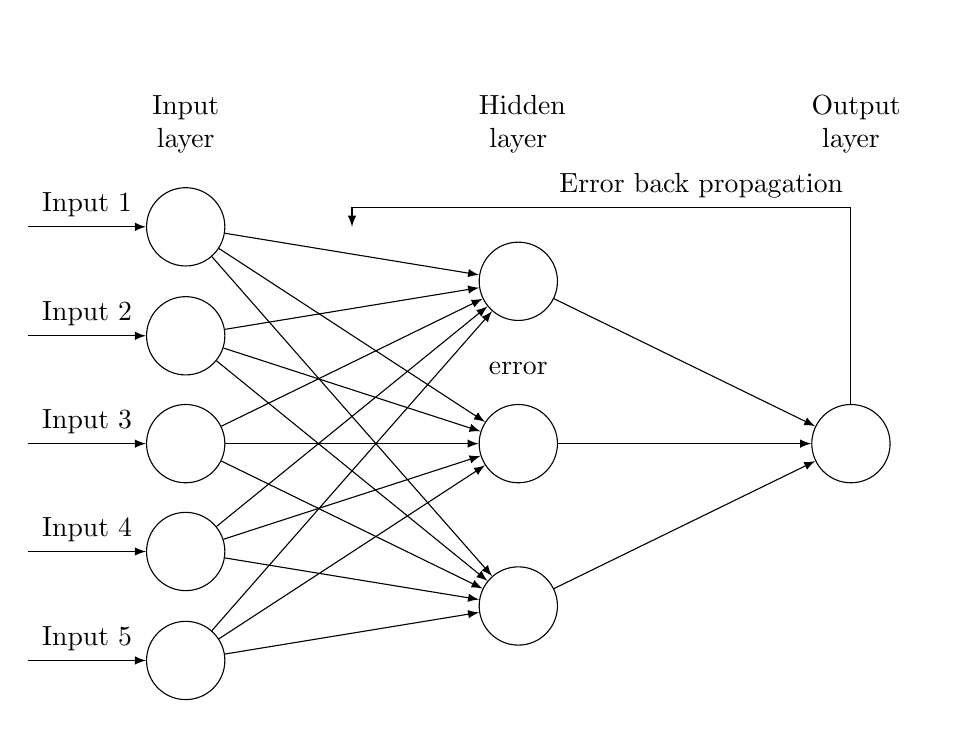
\begin{tikzpicture}[
    plain/.style={
      draw=none,
      fill=none,
      },
    net/.style={
      matrix of nodes,
     nodes={
       draw,
        circle,
    inner sep=10pt
    },
  nodes in empty cells,
  column sep=2cm,
  row sep=-9pt
  }, 
 >=latex
 ]
\matrix[net] (mat)
{ 
|[plain]| \parbox{1cm}{\centering Input\\layer} & |[plain]| \parbox{1cm}{\centering     Hidden\\layer} & 
|[plain]| \parbox{1cm}{\centering Output\\layer} \\
& |[plain]| \\
|[plain]| & \\
& |[plain]| \\
|[plain]| & |[plain]| \\
& & \\
|[plain]| & |[plain]| \\
& |[plain]| \\
|[plain]| & \\
& |[plain]| \\
};
\foreach \ai [count=\mi ]in {2,4,...,10}
  \draw[<-] (mat-\ai-1) -- node[above] {Input \mi} +(-2cm,0);
\foreach \ai in {2,4,...,10}
{\foreach \aii in {3,6,9}
  \draw[->] (mat-\ai-1) -- (mat-\aii-2);
}
\foreach \ai in {3,6,9}
  \draw[->] (mat-\ai-2) -- (mat-6-3);
%\draw[->] (mat-6-3) -- node[above] {Ouput} +(2cm,0);
\path [line] node{error} -- (mat-1-1);
\draw[->] (mat-6-3) -- ++(0pt,3cm) -| node[pos=0.15,above] {Error back propagation} ( $ 
(mat-2-1)!0.5!(mat-2-2) $ );
\end{tikzpicture}

\end{document}
